% Activate the following line by filling in the right side. If for example the name of the root file is Main.tex, write
% "...root = Main.tex" if the chapter file is in the same directory, and "...root = ../Main.tex" if the chapter is in a subdirectory.
 
%!TEX root =  

\chapter{Requirements Specification}\label{reqspec}

\minitoc

\subsection*{Purpose}
This requirements specification has been prepared for and accepted by SINTEF ICT (the customer) it states the requirements for the software system to be developed for the course TDT4290: Customer Driven Project. The requirements span two categories; functional requirements, describing the functionality the software needs to supply, and non-functional requirements, expected quality.

The requirement specification, once accepted by the customer, will serve as a contract between the parties involved, being a guideline for design and implementation and the standard against which the product is evaluated. It could also serve as a basis for further development of the Privacy Advisor system.

\section{Introduction}
\subsection{Background and Current Privacy Advising Software}
SINTEF ICT is currently investigating new approaches to privacy protection of end-users. T{\o}ndel et al. (2011) proposes a specific agent design for a machine learning approach to advice users on privacy actions based on:

\begin{itemize}
\item Past behavior using case based reasoning (CBR)
\item Similar users' behavior in similar situations using collaborative filtering (CF)
\end{itemize}

While there are systems for privacy protection, and more specifically aiding users in making privacy related decisions, the majority of these systems rely in a large extent on the user pre-specifying his preferences and being prompted with messages about where the policy of a given site conflicts with the user's preferences. Our design aims at being "low profile" or "non invasive'', that is able to make sensible decisions with as little interference as possible, and at the same time, given as little feedback as possible, able to cater for the dynamic nature of both web sites' privacy policies and user preferences with respect to privacy.

\subsection{Scope}\label{reqScope}

The primary aim of this project is the implementation of the core classification system described in T{\o}ndel et al. (2011) to allow for testing the applicability of the suggested approach to predicting privacy preferences. Since the software is intended to be a part of a research project, a design that allows for testing of various hypotheses and models is required. This implies a highly modular design where the various components of the core system can be replaced for the purpose of more detailed research. 

Furthermore, given the research nature of the project, less emphasis is placed on developing a complete stand-alone application. The core focus for our project will be on developing the underlying system and an interface for testing and parameter estimation. Hence development can take two directions:

\begin{enumerate}
\item A testing system that can be fed a knowledge base consisting of input-output mappings (P3p + context -> decision), and run interactive tests on a sample where the user is allowed to give feedback to the system and see the explanation for the recommendation. We envision a dual CLI/GUI (command line interface and graphical user interface) solution for this. In a final product, this testing system can also be used for the purpose of calibrating the model.
\item An end-user system that can run as a browser plug-in giving real time advice to the user as he browses the web.
\end{enumerate}

While theoretically appealing, there is little empirical research documenting the applicability of CBR to the task at hand, which in turn implies that there is likely a large research work to be done for the system to be able to successfully predict user preferences. Based on this observation, the emphasis of this project will be on the first of the above directions, namely providing a research framework.

\subsection{Overview}
This document is organized as follows:
�	Section~\ref{sysDesc} gives an overview over the system; its requirements and user characteristics.
�	Section~\ref{useCase} presents four different use-case scenarios.
�	Section~\ref{specRec} presents specific functional and non-functional requirements.
\section{Overall Description}

\section{System Description}\label{sysDesc}
The overall structure of the system is detailed in T{\o}ndel et al. (2011), and consists of the local CBR reasoning system, the remote/community collaborative filtering, both with their respective databases for storing information. This is in turn linked to an interface that is able to read and parse P3P policy files that are retrieved either from a local file (for the testing system) or by retrieving from the web.

\begin{figure}[htbp]
\begin{center}
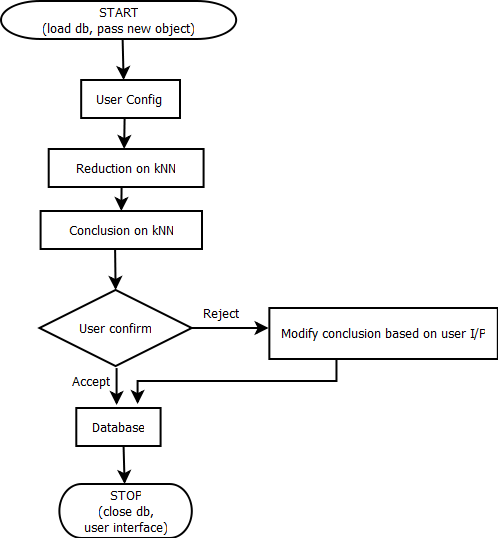
\includegraphics[width = \textwidth]{DesignReport/uml/flowchart.png}
\caption{Program Flow.}
\label{ReqSpecFlow}
\end{center}
\end{figure}

\subsection{User Interface}
Because of the research nature of the project, the customer considers the user interface to be of small importance. As the underlying algorithm/methodology is in an early development phase, the core focus is placed on producing a system for model testing and evaluation rather than an end user interface. 

\subsection{Hardware and Software Interface}
Being written in Java, the software requires a local copy of the Java Runtime Environment (JRE) installed on the computer. 

For the community functionality (collaborative filtering), a dedicated server running the filtering engine must also be available. Since this is basically a modified version of the local server, it has similar requirements, but as it presumably will hold a larger knowledge base, its hardware requirements will be greater, as both lookup time (computational demands) and storage demands will increase with the number of users. It may also require additional server/database software such as mySQL, CouchDB etc. 

\subsection{User Characteristic}

For this project we distinguish between two groups constituting the users of the product. 
\subsubsection{Developers/Researchers}
Firstly, developers/researchers that will be working on the testing and calibration of the underlying model and extending it to other policy types beside P3P etc. These users are the primary focus of our work. A research/developer is an expert user, and needs to be familiar with how privacy policies are coded in machine-readable form such as P3P, but also the software source codes in order to modify, extend and optimize the algorithms. 

\subsubsection{End Users}
Secondly, the end user who will be using the software in the form of a browser plugin that provides advice with respect to the users behavior on the Internet. A key objective for the project is that the agent is to be able to make good decisions and require as little feedback as possible from the user. To the extent interaction is needed, it should be able to clearly state an explanation for its decisions and allow the user to override in a simple manner.


\section{Use Cases}\label{useCase}

The first use case illustrates a research setting where calibration/testing interface allows the user to load in a dataset of P3P policies and test the performance of the underlying model. The last three use cases illustrate the potential application of the system as a browser plugin that runs in the background monitoring the users activities and the web sites he is visiting. As previously stressed, the success of testing according to the first use case determines the extent to which the system described in cases 2-4 is implemented.

\subsection*{Case 1: Research/calibration}
In this case a researcher wants to test the properties of the underlying model. Using the Calibration GUI, he imports 50 P3P policies that are parsed. Further he designates that 40 of these are to be stored immediately in the knowledge base along with a corresponding action for each policy.

The user now specifies the distance metric he wants to apply to each of the different components. Finally, he can either set the (importance) weights assigned to each of the policy components, or he can load the weights from a flat text file. Now that the configuration is complete, the ten policies withheld earlier from the sample can be classified. For each of the ten policies, the user can choose either to accept, or reject, and provide a reason for his rejection before proceeding to the next policy. 

\subsection*{Case 2: End user - local query, recommendation accepted, site rejected}
A user visits a previously unvisited website. The privacy agent tries to retrieve machine-readable privacy information from the site. When the policy is obtained it is parsed and a context object, consisting of the policy, domain, time of visit, and other contextual information, is created. The context object is compared to the local database for similar contexts. Since the user has visited sites with a similar policy previously, the comparison succeeds and the site is blocked based on data from the local database. The user agrees with this decision and navigates away from the site.

\subsection*{Case 3: End user - local query, site approved by recommender, recommendation accepted}
A user visits a previously unvisited website. As before, the system fetches the necessary data to do a local query. This query indicates, with sufficient confidence, that the site's policy is acceptable. The user is then allowed to continue browsing with no intervention from the Privacy Agent.

\subsection*{Case 4: End user - global query, recommendation overridden}
As before, but in this case, no sufficiently similar cases are found locally. In this case the system will query the global server for similar users that have visited the same site to base its decision on this. In this case, site is blocked, but the user disagrees. He selects an override feature and gives a reason for why he overrides.

\section{Specific Requirements}\label{specRec}

\subsection{Product perspective}
As described in Section~\ref{reqScope}, as the main goal of the project is to develop a testing framework for the core reasoning system. The secondary goal is to implement a user interface that can work as a stand-alone application to allow for actual user testing.

\subsection{Functional Requirements}
\begin{itemize}

\item The system should be able to parse a P3P file to instantiate the data as a privacy case/event/instance.
\item Based on past history (knowledge base), it should retrieve the cases most similar to the one presented.
\item Given the degree of similarity to past cases and the uniformity of action taken in the past, the system can either 
  \begin{itemize}
  \item Give the user a recommendation or 
  \item Pass the recommendation decision on to the community/CF system.
  \end{itemize}
\item If passed on to the CF, the system will query a server for the most similar users and use the data on their decisions in similar cases to make a recommendation (along with local/CBR recommendation) 
\item Update the database with the recommendation.
\item Allow the user to view the explanation for the recommendation
\item Allow the user to overrule a recommendation. 
\item When overruling a recommendation, the user must be allowed to explain why the decision is made, e.g. one time occurrence, permanent rule, etc.	
\item Allow the user, if making a new general rule, to backtrack and alter previous cases
\end{itemize}

\subsection{Non-Functional Requirements}
\begin{itemize}
\item Implementation
  \begin{itemize}
  \item Code is written in Java following Sun Microsystems' conventions\footnote{http://www.oracle.com/technetwork/java/codeconvtoc-136057.html}.
  \item Third party libraries are to be documented with version numbers and to be included in the installation package.
\end{itemize}

\item Maintainability:
  \begin{itemize}
  \item Code repositories and version control: github is used as code repository and for version control.
  \item User documentation is to be produced.
  \item A well documented API is to be designed	
  \item English (US) is to be used as language for naming convention for source code and filenames, and in code comments and documentation.
  \item The code is to be designed in a modular fashion.
  \end{itemize}

\item Performance: 
  \begin{itemize}
  \item For the final end-user product that will run as a browser plug-in, performance will be important, as the program should not be seen as a nuisance in getting work done.
  \end{itemize}

\item Portability: 
  \begin{itemize}
  \item The testing/design system should be portable to any system with a JRE.
  \end{itemize}

\item User interface:
  \begin{itemize}
  \item Two UIs are to be implemented: A command line interface (CLI) as well as a GUI is to be designed using Java/swing.
  \item These interfaces are meant to facilitate testing the model framework.
  \end{itemize}


\end{itemize}
